\section{Comparaison de branches sans ramifications}
\begin{frame}{Format PDB et représentation}
    \footnotesize
    \begin{figure}[!htb]
        \centering
        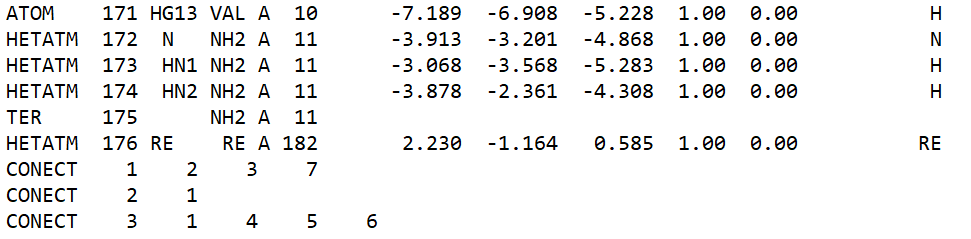
\includegraphics[width=9cm]{lignes_pdb}
        \caption{\label{fig:pdb}Lignes d'un fichier PDB}
    \end{figure}
    \begin{minipage}{0.45\textwidth}%
    \begin{center}
        \underline{Données}
    \end{center}
    \begin{tabular}{ccc}
    position des atomes & $\rightarrow$ & OK \\
    type des atomes & $\rightarrow$ & OK \\
    liaisons & $\rightarrow$ & moyennes
    \end{tabular}
    \end{minipage}%
    \hfill
    \begin{minipage}{0.45\textwidth}%
    \begin{figure}[!htb]
        \centering
        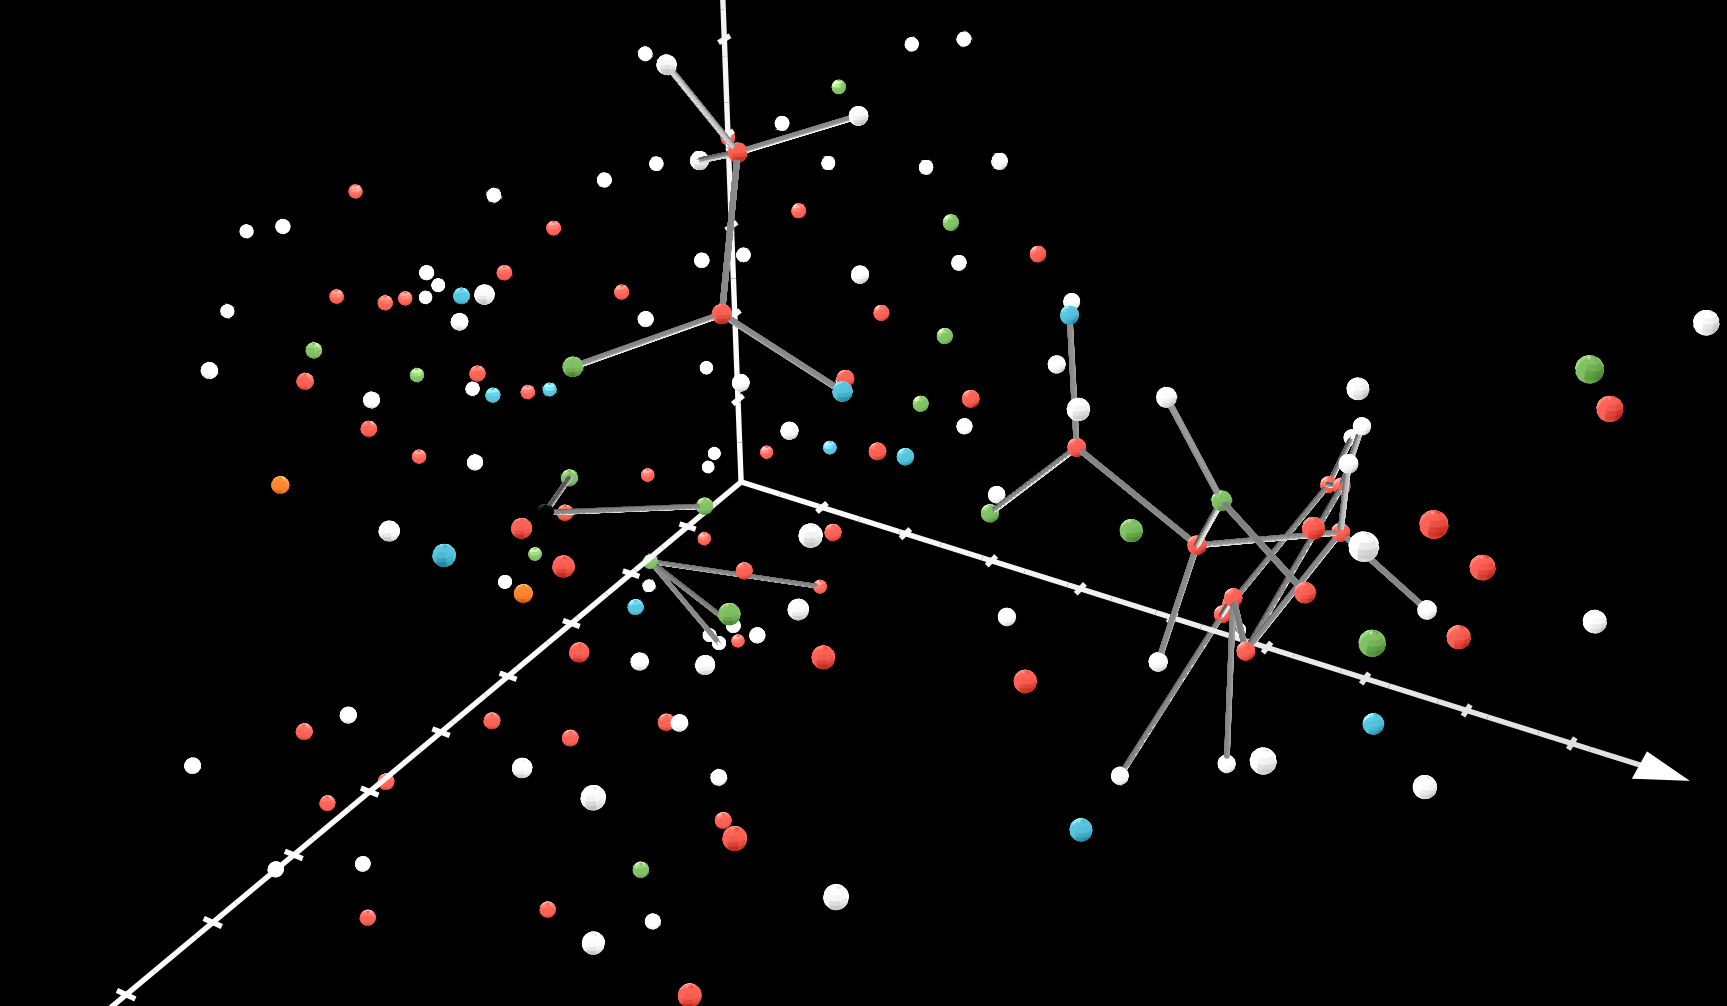
\includegraphics[width=4cm]{protein_peuliaisons_pres}
    \end{figure}
    \end{minipage}%
\end{frame}

\subsection{Notion de branche}
\begin{frame}{Branche sans ramification}
    \begin{minipage}{0.5\textwidth}%
        \begin{figure}[!htb]
            \centering
            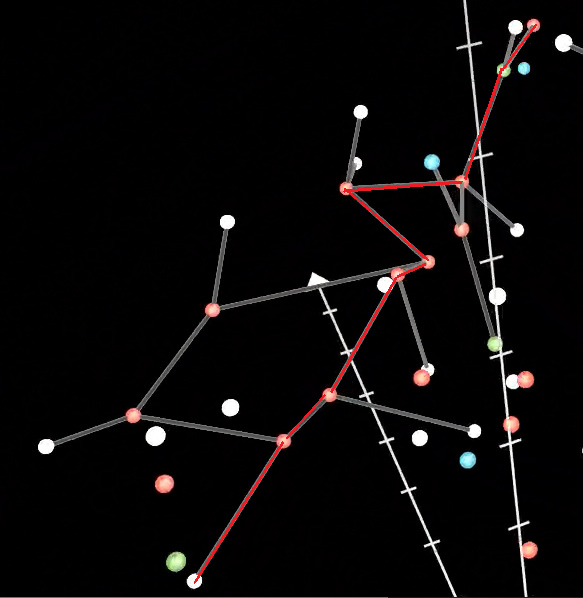
\includegraphics[width=5.5cm]{protein_branche}
        \end{figure}
    \end{minipage}%
    \hfill
    \begin{minipage}{0.4\textwidth}%
        \begin{figure}[!htb]
            \centering
            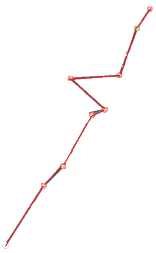
\includegraphics[width=3cm]{branche_extraite}
        \end{figure}
    \end{minipage}%
    \newline \newline \newline
    \underline{en python} : 
    \begin{itemize}
        \item type : \textcolor{airforceblue}{Coord} : $float\ *\ float\ *\ float$
        \item type : \textcolor{airforceblue}{Branche} : liste de points 
            \newline \underline{ex} : $B = [(0,0,0), (1,1,1), (1.5,1,2)]$
    \end{itemize}
\end{frame}

\subsection{Comparaison}
\begin{frame}{Comparaison de branches : distances}
    \begin{minipage}{0.45\textwidth}%
        \begin{figure}[!htb]
            \centering
            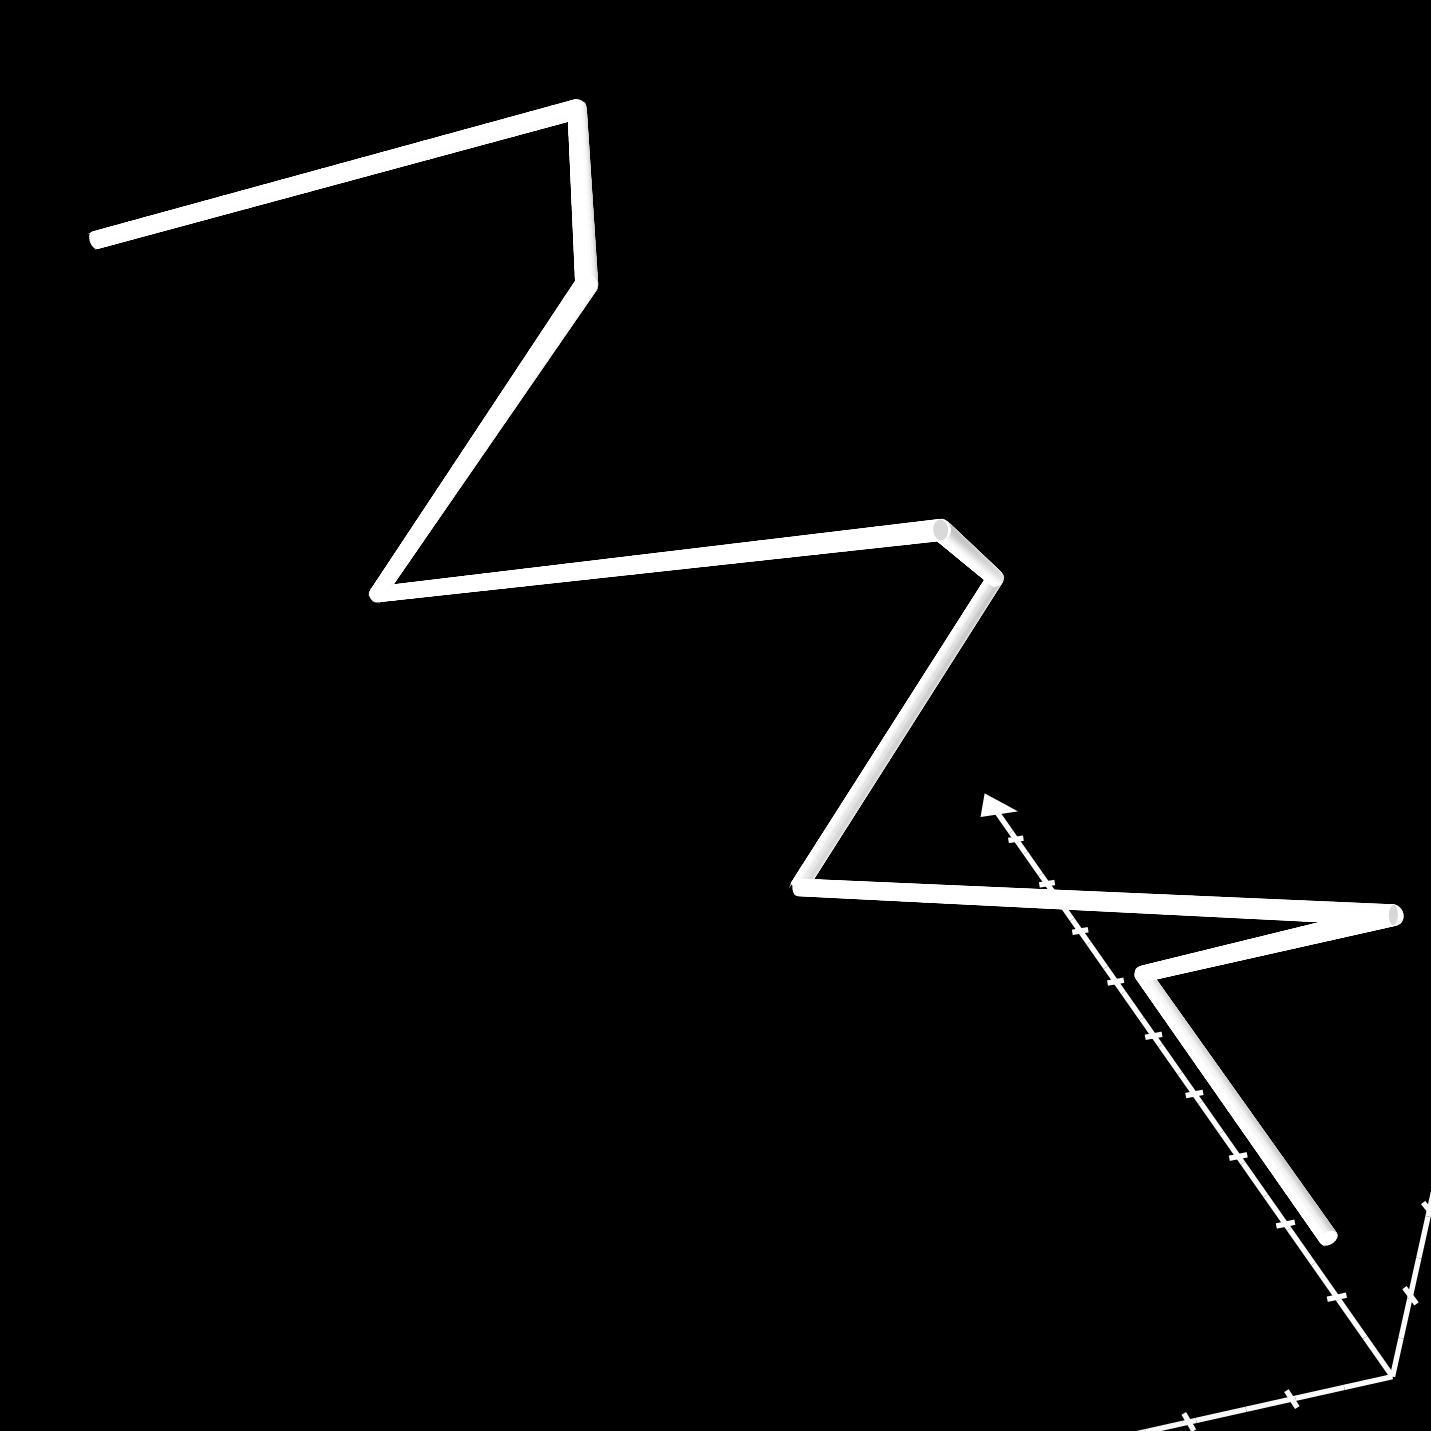
\includegraphics[width=3cm]{branche_white}
            \caption{\label{fig: b_white} Branche A}
        \end{figure}
        \begin{figure}[!htb]
            \centering
            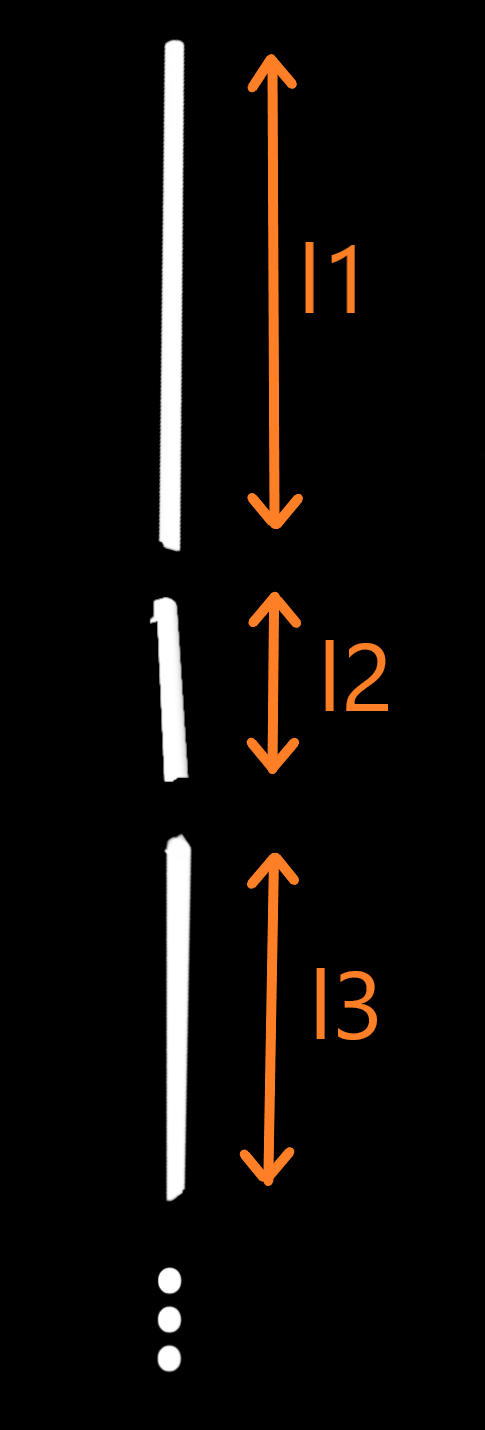
\includegraphics[width=1.3cm]{li}
        \end{figure}
    \end{minipage}%
    \hfill
    \begin{minipage}{0.45\textwidth}%
        \begin{figure}[!htb]
            \centering
            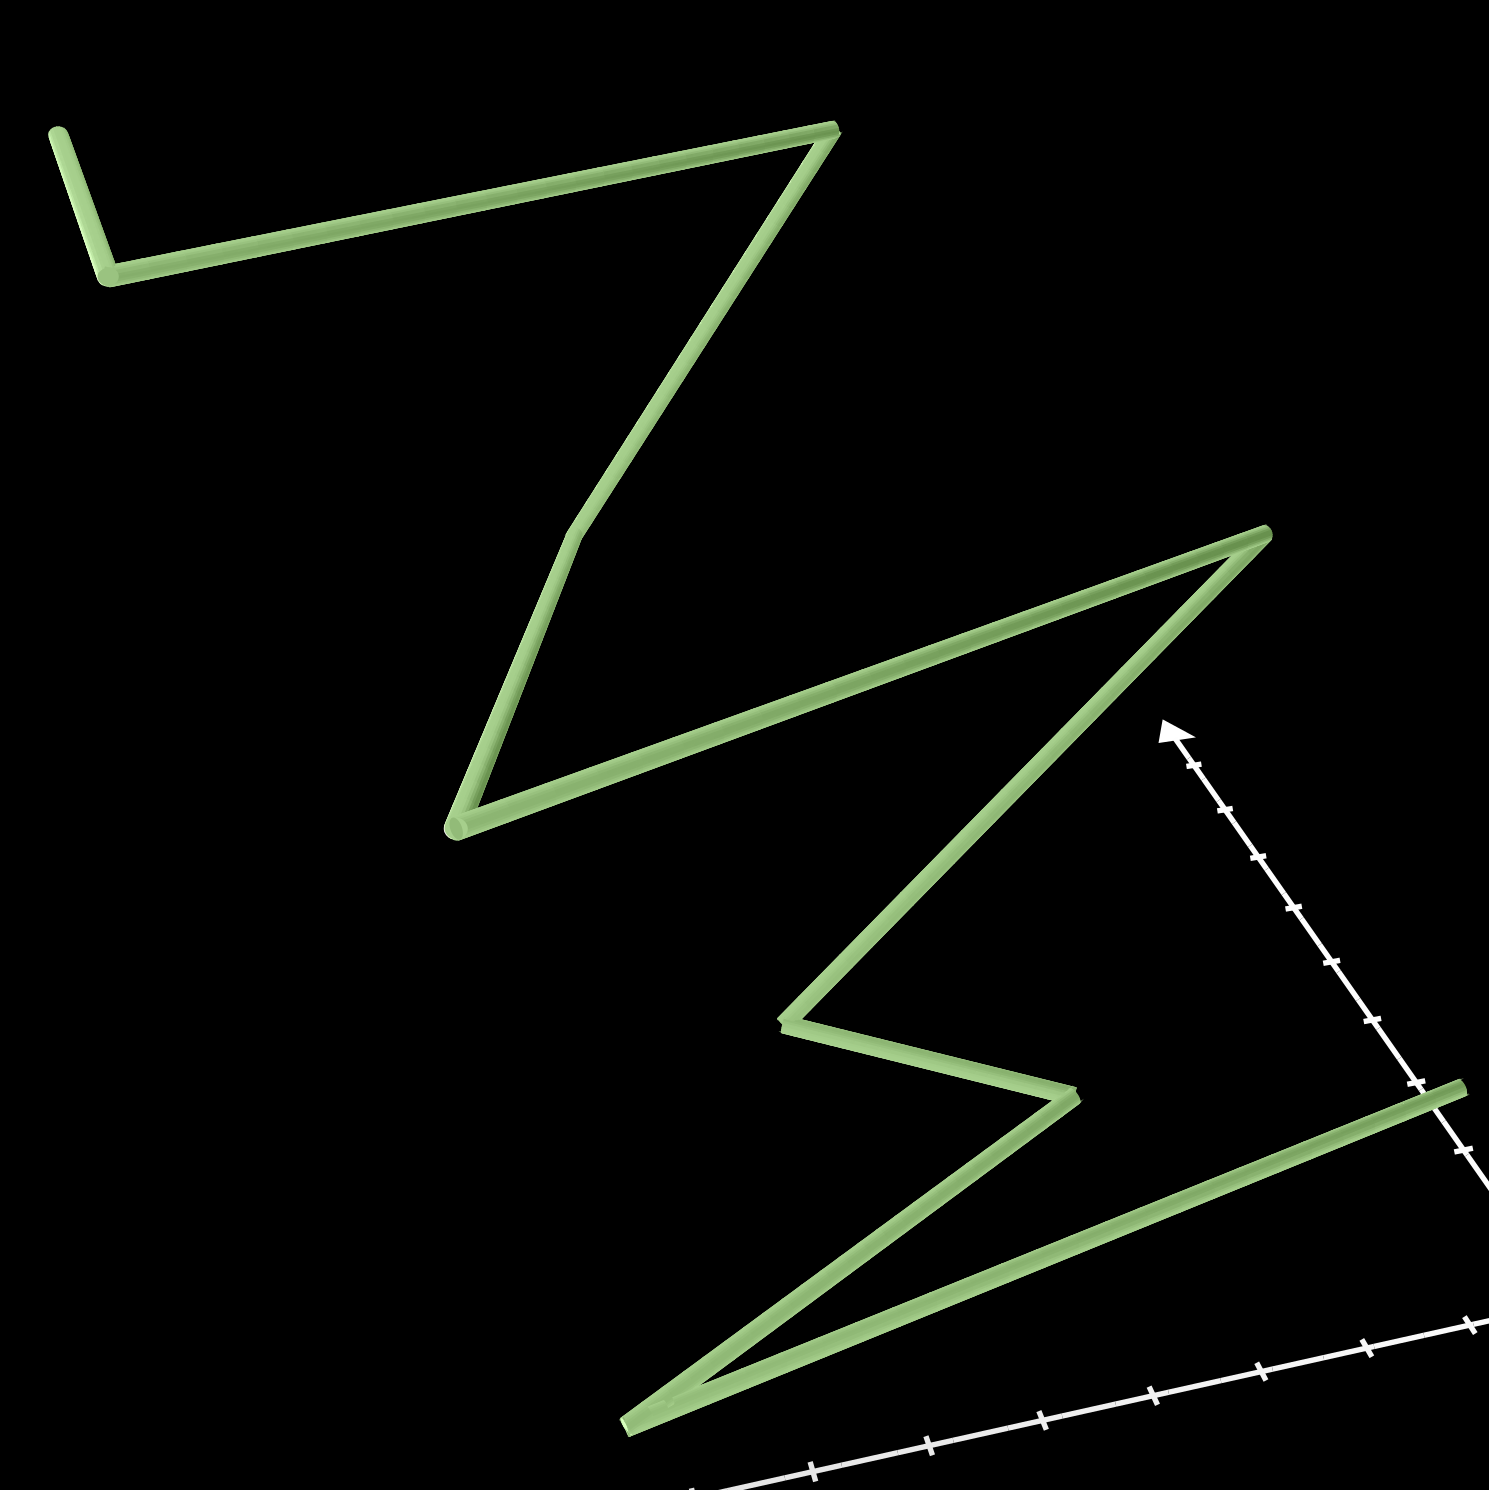
\includegraphics[width=3cm]{branche_green}
            \caption{\label{fig: b_green} Branche B}
        \end{figure}
        \begin{figure}[!htb]
            \centering
            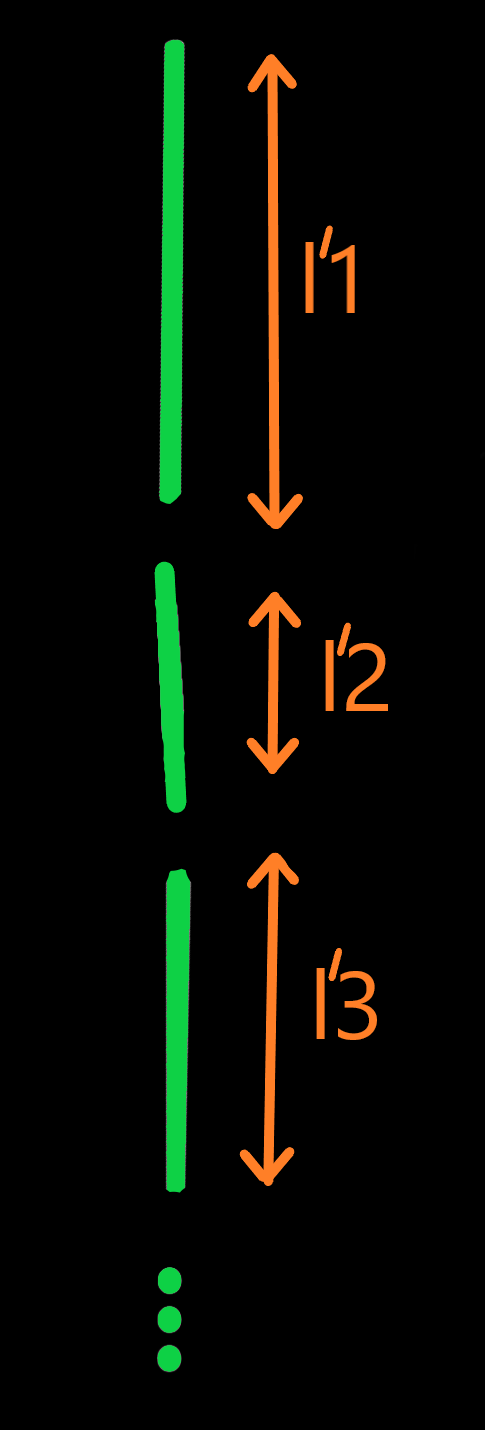
\includegraphics[width=1.3cm]{lprimei}
        \end{figure}
    \end{minipage}%
\end{frame}

\begin{frame}{Comparaison de branches : angles}
    \begin{multicols}{2}
        \begin{figure}[!htb]
            \centering
            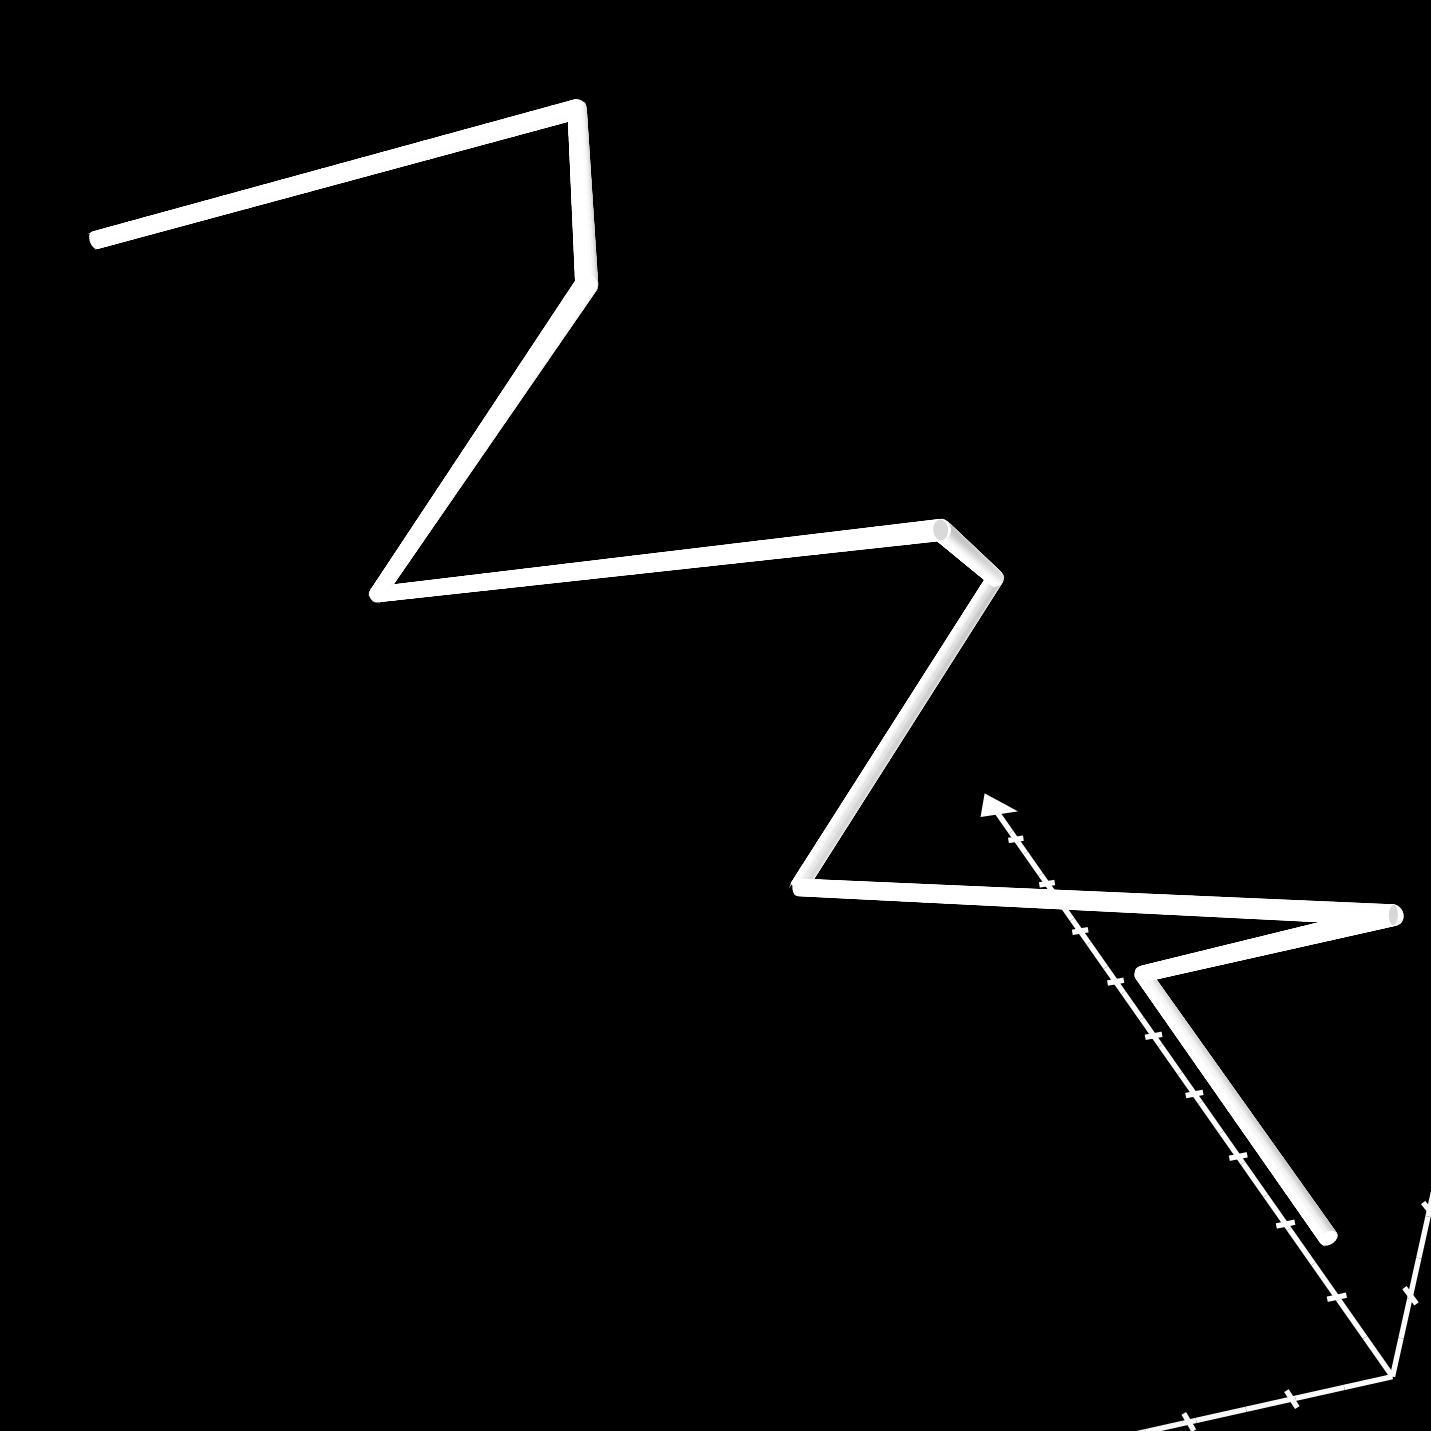
\includegraphics[width=3cm]{branche_white}
            \caption{\label{fig: b_white2} Branche A}
        \end{figure}
        \begin{figure}[!htb]
            \centering
            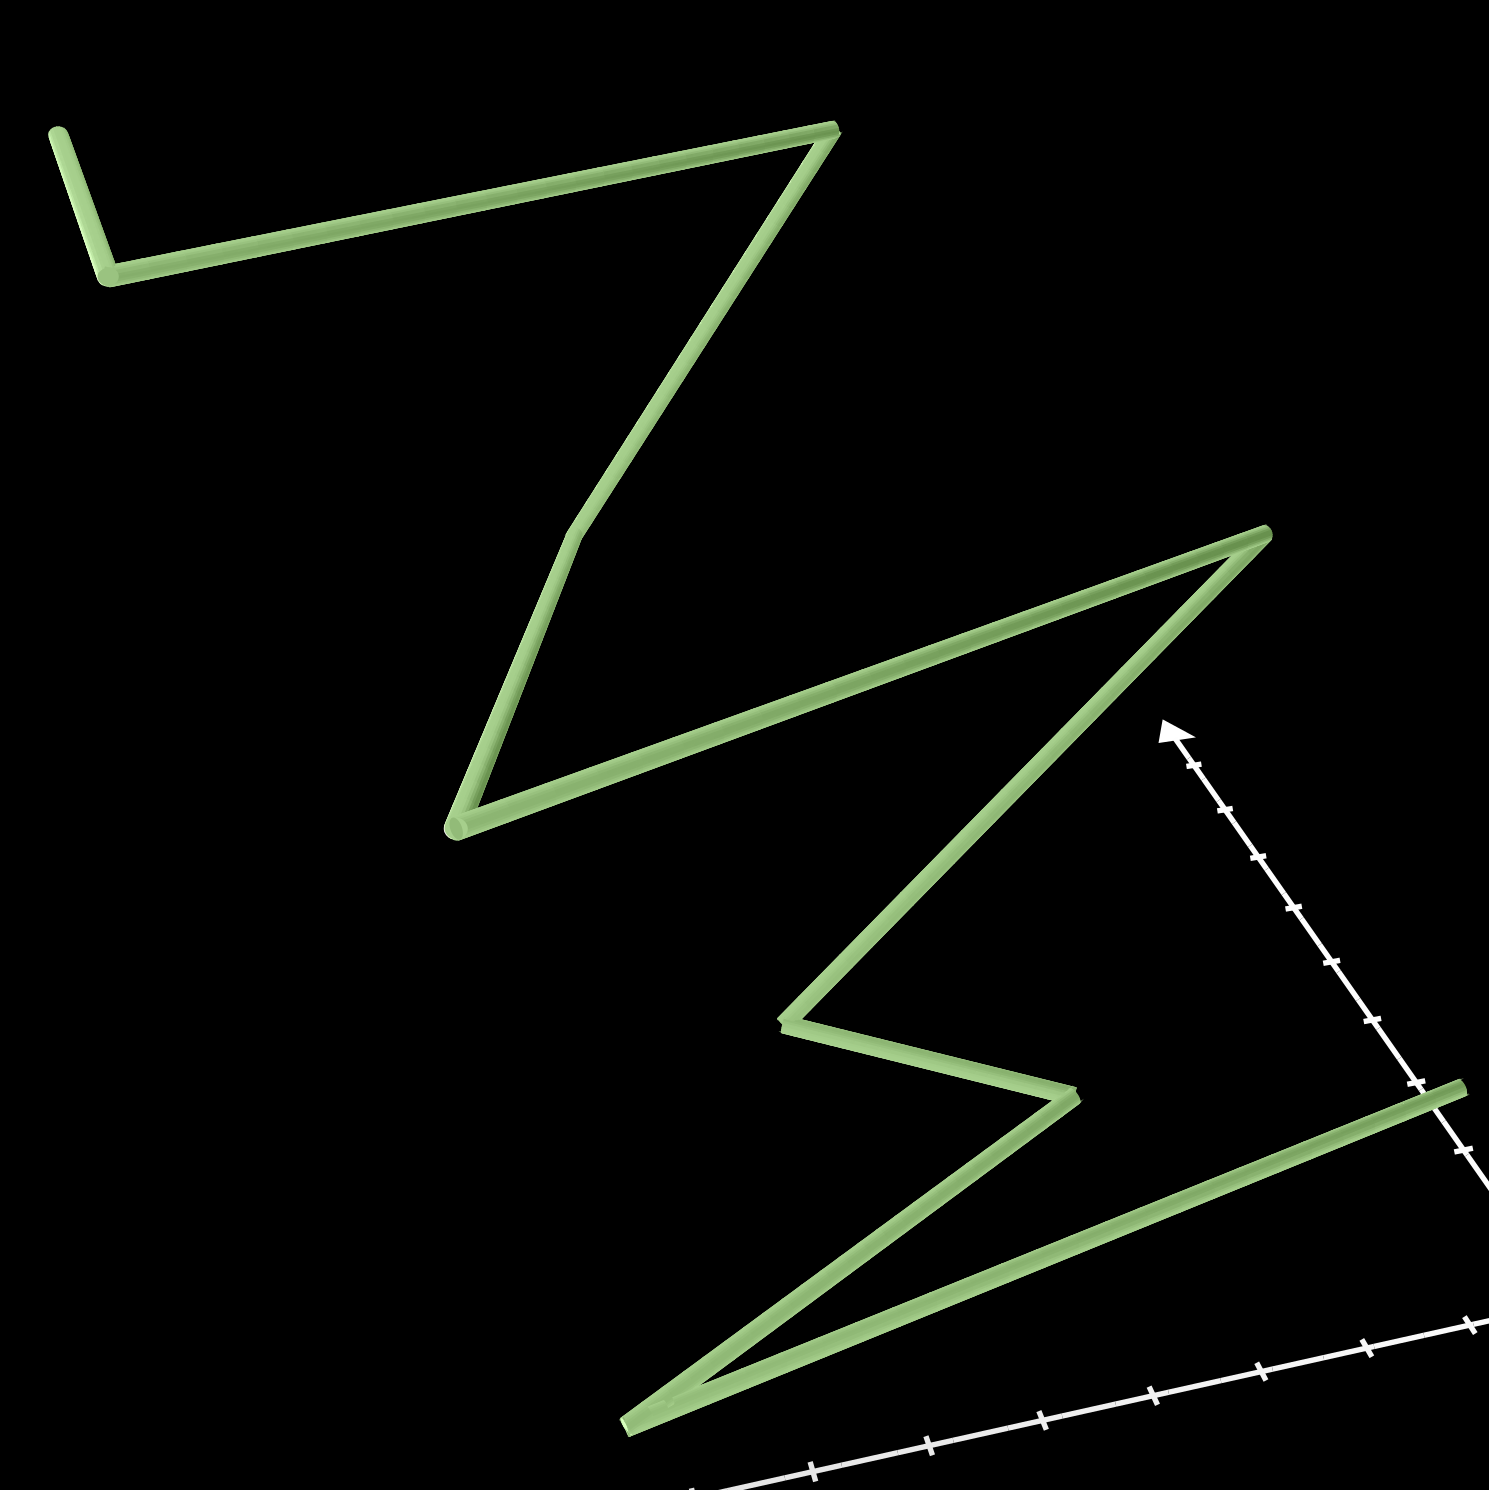
\includegraphics[width=3cm]{branche_green}
            \caption{\label{fig: b_green2} Branche B}
        \end{figure}
    \end{multicols}
    \begin{figure}[!htb]
        \centering
        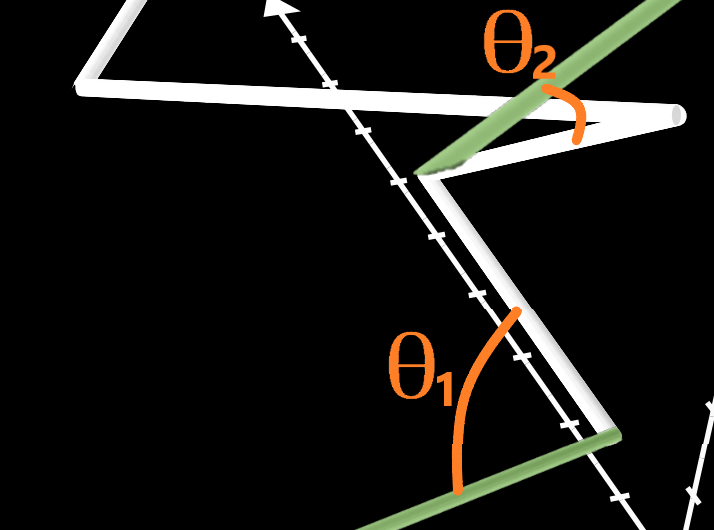
\includegraphics[width=3cm]{thetai}
        \caption{\label{fig: thetai} Angles}
    \end{figure}
\end{frame}

\subsection{Coefficient}

\begin{frame}{Coefficient de proximité de branches}
    \begin{align*}
    \forall i \in [\![1,n-1]\!],\ d_i = max(l_i,l_i') \\
    \end{align*}
    \begin{equation*}
        C_{dist} = \frac{\displaystyle\sum_{i=0}^{n-1} | \sin(\theta_{i}) | d_i}{\displaystyle\sum_{i=0}^{n-1} d_i} \qquad  
        C_{angle} = \frac{\displaystyle\sum_{i=0}^{n-1} |l_i' - l_i|}{\displaystyle\sum_{i=0}^{n-1} d_i}
    \end{equation*}
    \begin{equation*}
        R_{dist} = \frac{1}{1 + C_{dist}} \qquad R_{angle} = \frac{1}{1 + C_{angle}}
    \end{equation*}
    \newline Finalement, on définit : \newline
    \begin{equation*}
        \boxed{R = \frac{R_{dist}+R_{angle}}{2}}
    \end{equation*}
\end{frame}

\begin{frame}{Valeur du coefficient sur exemples}
    \begin{multicols}{2}
        \begin{figure}
            \centering
            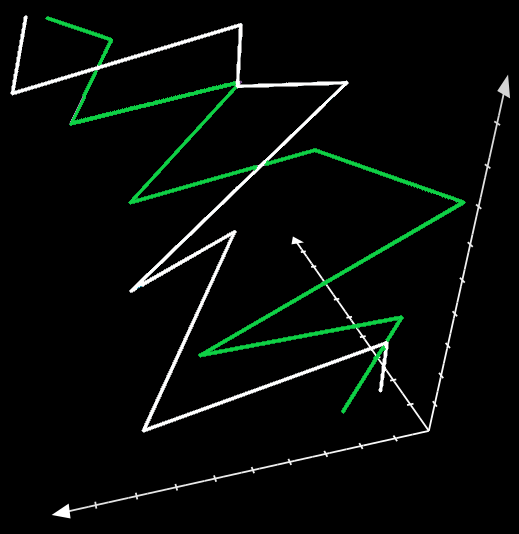
\includegraphics[width=3.5cm]{rcoeff_dist059_ang068_tot064_2}
        \end{figure}
    \vspace*{0.2cm}
        \begin{align*}
            R_{dist} = &0.59 \quad R_{angle} = 0.68 \\
            &\boxed{R = 0.64}
        \end{align*}
    \end{multicols}
    \begin{multicols}{2}
        \begin{figure}
            \centering
            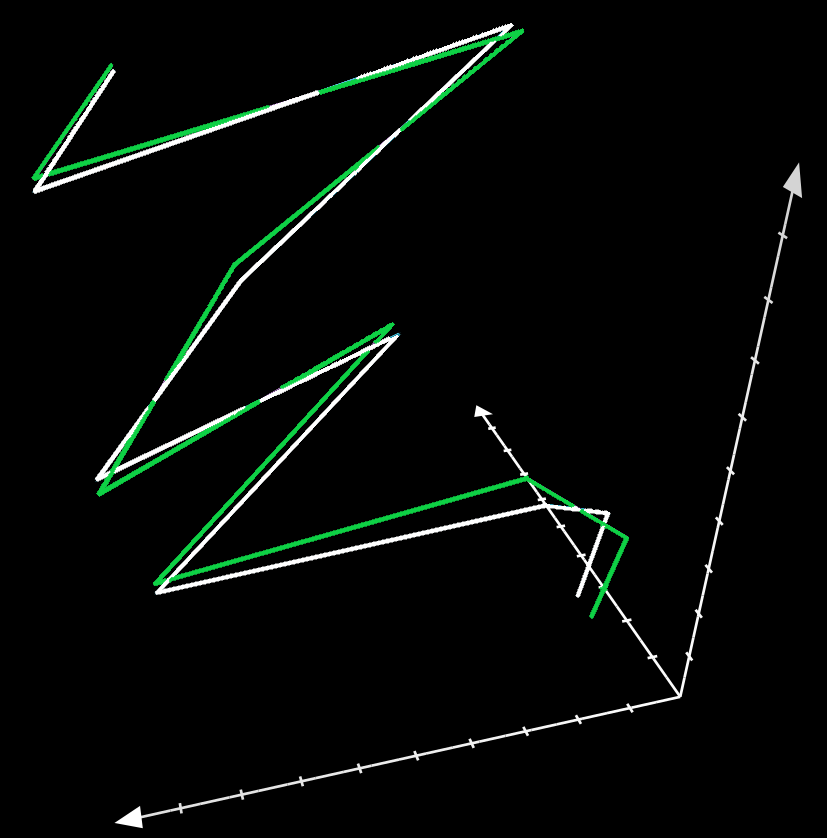
\includegraphics[width=3.5cm]{rcoeff_dist094_ang097_tot095_2}
        \end{figure}
    \vspace*{0.2cm}
            \begin{align*}
                R_{dist} = &0.94 \quad R_{angle} = 0.97 \\
                &\boxed{R = 0.95}
            \end{align*}
    \end{multicols}
\end{frame}